\documentclass[11pt,letterpaper]{article}

\usepackage{amsmath}%
\usepackage{amsfonts}%
\usepackage{amssymb}%
\usepackage{dsfont}
%\usepackage{graphicx}
%\usepackage[latin1]{inputenc} 
%\usepackage[T1]{fontenc} 
%\usepackage{layout}
%\usepackage{setspace}
\usepackage{pgf,tikz}
\usepackage{subcaption}
\captionsetup{compatibility=false}
\usepackage[]{algorithm2e}
\usepackage{enumitem}
\usepackage[left=2.6cm,right=2.6cm,top=2cm,bottom=3cm]{geometry}
\usepackage{authblk}





\usetikzlibrary{decorations}
\usetikzlibrary{decorations.pathmorphing}
\usetikzlibrary{decorations.pathreplacing}
\usetikzlibrary{decorations.shapes}
\usetikzlibrary{decorations.text}
\usetikzlibrary{decorations.markings}
\usetikzlibrary{decorations.fractals}
\usetikzlibrary{decorations.footprints}

\usetikzlibrary{arrows}

\newtheorem{theorem}{Theorem}
\newtheorem{definition}{Definition}
\newtheorem{lemma}{Lemma}
\newtheorem{example}{Example}
\newtheorem{corollary}{Corollary}
\newtheorem{problem}{Problem}
\newtheorem{acknowledgement}[theorem]{Acknowledgement}
\newtheorem{axiom}[theorem]{Axiom}
\newtheorem{case}[theorem]{Case}
\newtheorem{claim}[theorem]{Claim}
\newtheorem{conclusion}[theorem]{Conclusion}
\newtheorem{condition}[theorem]{Condition}
\newtheorem{conjecture}[theorem]{Conjecture}

\newtheorem{criterion}[theorem]{Criterion}
\newtheorem{exercise}[theorem]{Exercise}
\newtheorem{notation}[theorem]{Notation}
\newtheorem{proposition}[theorem]{Proposition}
\newtheorem{remark}[theorem]{Remark}
\newtheorem{solution}[theorem]{Solution}
\newtheorem{summary}[theorem]{Summary}
\newenvironment{proof}[1][Proof]{\textbf{#1.} }{\ \rule{0.5em}{0.5em}}

\newcommand{\kctp}{$k$-CTP}
\newcommand{\set}[1]{\left\{ #1 \right\}}
\newcommand{\card}[1]{\left| #1 \right|}
\newcommand{\ith}[1]{#1^{\mbox{\scriptsize{th}}}}
\newcommand{\stpath}{$(s,t)$-path}
\newcommand{\stpaths}{$(s,t)$-paths}
\newcommand{\true}{\mbox{true}}
\newcommand{\false}{\mbox{false}}
\newcommand{\ifend}{\textbf{endif}}
\newcommand{\karp}{=_{\mbox{\scriptsize{K}}}}
\newcommand{\lkarp}{\leq_{\mbox{\scriptsize{K}}}}
\newcommand{\omegamin}{\omega_{\mbox{\scriptsize{min}}}}
\newcommand{\mcale}{\mathcal{E}}
\newcommand{\mcals}{\mathcal{S}}
\newcommand{\mcala}{\mathcal{A}}
\newcommand{\mcalv}{\mathcal{V}}
\newcommand{\mcalg}{\mathcal{G}}
\newcommand{\mts}{MS}
\newcommand{\mctp}{M-CTP}
\newcommand{\argmin}[1]{\underset{#1}{\operatorname{argmin}}}
\newcommand{\deltavert}{\Delta_{\mbox{\scriptsize{vert}}}}
\newcommand{\Gv}{G^{(v)}}
\newcommand{\Gvu}{G_{\mbox{\scriptsize{up}}}^{(v)}}
\newcommand{\Gvd}{G_{\mbox{\scriptsize{down}}}^{(v)}}
\newcommand{\betakmin}{\beta_{k}^*}
\newcommand{\pup}{p_A^{\mbox{\scriptsize{up}}}}
\newcommand{\pdown}{p_A^{\mbox{\scriptsize{down}}}}
\newcommand{\pdownbis}{p_{A'}^{\mbox{\scriptsize{down}}}}
\newcommand{\caup}{c_A^{\mbox{\scriptsize{up}}}}
\newcommand{\cadown}{c_A^{\mbox{\scriptsize{down}}}}
\newcommand{\cadownbis}{c_{A'}^{\mbox{\scriptsize{down}}}}


\title{Canadians should use memory}
\date{}
\author[,1]{Pierre Berg\'e \thanks{Corresponding author: \texttt{Pierre.Berge@lri.fr}}} 
\author[2]{Julien Hemery}
\author[2]{Arpad Rimmel}
\author[2]{Joanna Tomasik}
\affil[1]{LRI, Universit\'e Paris-Sud, Universit\'e{} Paris-Saclay, 91405 Orsay Cedex, France}
\affil[2]{LRI, CentraleSup\' elec, Universit\'e{} Paris-Saclay, 91405 Orsay Cedex, France}

\begin{document}


%\authorrunning{P. Berg\'e, A. Rimmel and J. Tomasik}

%\Copyright{P. Berg\'e, A. Rimmel and J. Tomasik}

\maketitle

\begin{abstract}
 
%The $k$-Canadian Traveller Problem, defined and proven PSPACE-complete by Papadimitriou and Yannakakis, is a generalization of the Shortest Path Problem which admits blocked edges. Its objective is to determine the strategy that makes the traveller traverse graph $G$ between two given nodes $s$ and $t$ with the minimal distance, knowing that at most $k$ edges are blocked. The traveller discovers that an edge is blocked when arriving at its endpoint. Westphal showed that the competitive ratio, which is an indicator of the online algorithm quality, of any randomized strategy is not less than $k+1$. 
 
%We study the competitiveness of randomized memoryless strategies for the \kctp . In this context, a decision taken by the traveler in node $v$ of $G$ does not depend on its anterior moves. 
We establish that the competitive ratio of any randomized memoryless strategy is not less than $2k+1$. Only randomized strategies using memory potentially overpass this ratio now.

%MThis means that a randomized strategy achieving the competitive ratio below this bound incorporates information about the previous moves of the traveller. The primordial consequence of this result is that, if we aim at designing a strategy such that its competitive ratio is smaller than $1.268 k +1$, we shall focus on strategies which are not memoryless.
\end{abstract}

\section{Definitions} \label{sec:def}

We start by introducing the notation. For any graph $G=\left(V,E,\omega\right)$, let $G\backslash E'$ denotes its subgraph $\left(V,E\backslash E',\omega\right)$. If $P$ is a path, we note its cost as $\omega\left(P\right) = \sum_{e \in P} \omega(e)$. 

\subsection{Memoryless Strategies for the \kctp} \label{subsec:msintro}

We remind the definition of CTP. Let $G=\left(V,E,\omega\right)$ be an undirected graph with positive weights. The objective is to make a traveller traverse the graph from a source node $s$ to a target one $t$, with $s,t \in V$. There is a set $E_* \subsetneq E$ of blocked edges. %Without blocked edges, the remaining graph can be still traversed by the traveller: there exists a \stpath ~in graph $G\backslash E_* = \left(V,E\backslash E_*\right)$. 
The traveller does not know a priori which edges are blocked. He discovers a blocked edge only when arriving to one of its endpoints. For example, if $\left(v,w\right)$ is a blockage he will discover it when arriving to $v$ (or $w$). The goal is to design the strategy $A$ with the minimal competitive ratio.

\begin{figure}[t]
\centering
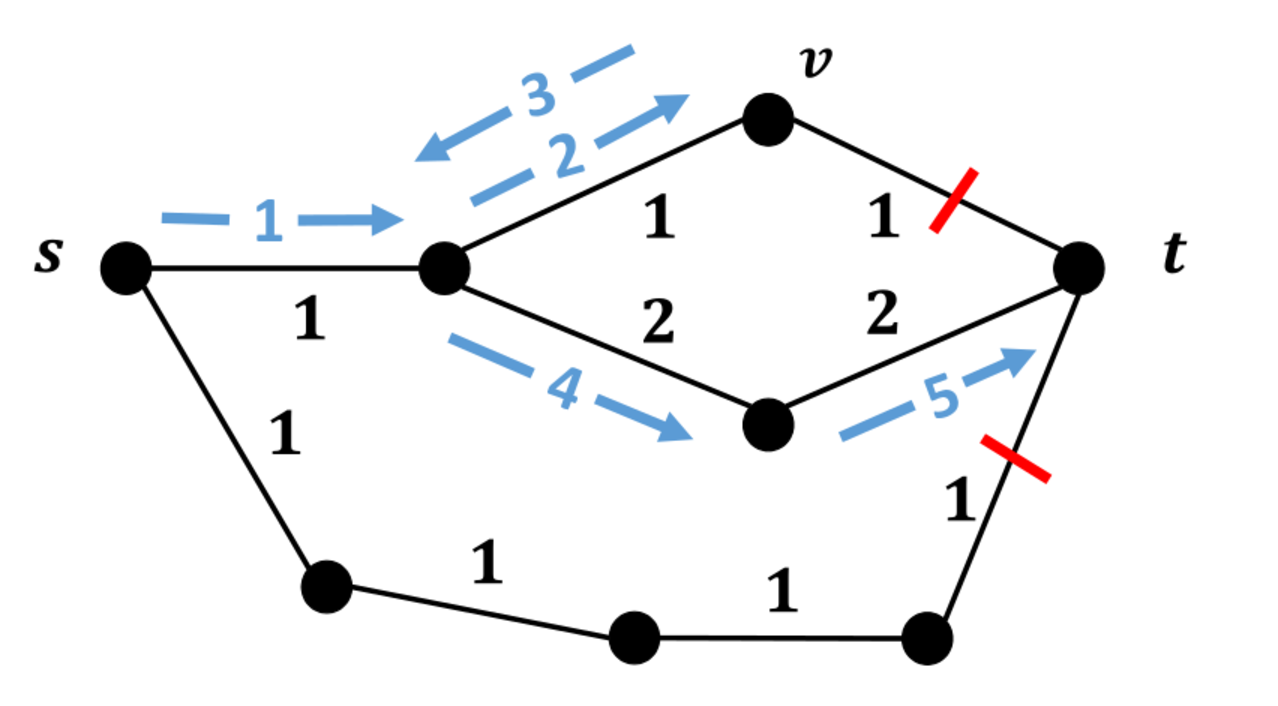
\includegraphics[scale=0.27]{illustrateCTP2.pdf}
\caption{Illustration of the \textsc{greedy} strategy on a graph with 2 blocked edges}
\label{fig:illustrateCTP}
\end{figure}

We focus on \textit{memoryless strategies} (\mts). Concretely, we suppose that the traveller remembers the blocked edges he has discovered but forgets the nodes which he has already visited. In other words, a decision of an \mts ~is independent of the nodes already visited. In the literature, the term \textit{memoryless} was used in the context of online algorithms (e.g. \textsc{paging problem}~\cite{BoEl98}, \textsc{list update problem}~\cite{Al03}) which take decisions according to the current state, ignoring past events. An \mts ~can be either deterministic or randomized.



\begin{definition}[Memoryless Strategies for the \kctp]
A deterministic strategy $A$ is an \mts ~if and only if (iff) the next node $w$ the traveller visits depends on graph $G$ deprived of blocked edges already discovered $E_*'$ and the current traveller position $v$: $w = A\left(G\backslash E_*',v\right)$. Similarly, a randomized strategy $A$ is an \mts ~iff node $w$ is the realization of a discrete random variable $X = A\left(G\backslash E_*',v\right)$.
\end{definition}

\mts es are easy to be implemented because they do not use past moves to take a decision.  For the same reason, they do not need any extra memory either.

For example, the \textsc{greedy} strategy~\cite{XuHuSuZh09} is an \mts . It consists in choosing at each step the first edge of the shortest path between the current node $v$ and the target~$t$. This strategy, illustrated in Figure~\ref{fig:illustrateCTP}, does not refer to anterior moves. In contrast, the \textsc{reposition} strategy~\cite{We08} is not an \mts ~as any decision refers to the past moves of the traveller. 

We propose the following process to identify whether a strategy $A$ is a deterministic \mts . Let us suppose that a traveller $T_1$ executes strategy $A$: he has already visited certain nodes of the graph, he is currently at node $v$ but he has not reached target $t$ yet. Let us imagine a second traveller $T_2$ who is airdropped on node $v$ and starts applying strategy $A$. If the traveller $T_2$ always follows the same path as $T_1$ until reaching $t$, $A$ is a deterministic \mts . If $T_1$ and $T_2$ may follow different paths, then $A$ is not an \mts . Formally, prooving that a strategy is an \mts ~consists in finding the function which transforms the pair $\left(G\backslash E_*,v\right)$ into node $w = A\left(G\backslash E_*',v\right)$.

\subsection{Competitive ratio} \label{subsec:compratio}

Let $\left(G,E_*\right)$ be a \textit{road map}, {\em i.e.} a pair with graph $G=\left(V,E,\omega\right)$ and blocked edges $E_* \subsetneq E$, such that there is an \stpath ~in graph $G\backslash E_*$ (nodes $s$ and $t$ always remain in the same connected component). We note $\omega_A\left(G,E_*\right)$ the distance traversed by the traveller reaching $t$ with strategy $A$ on graph $G$ with blocked edges $E_*$ and $\omegamin\left(G,E_*\right)$ the cost of the shortest \stpath ~in graph $G\backslash E_*$.

The ratio $\omega_A\left(G,E_*\right)/\omegamin\left(G,E_*\right)$ is abbreviated as $c_A\left(G,E_*\right)$. A strategy $A$ is $c_A$-competitive~\cite{BoEl98,XuHuSuZh09} iff for any $\left(G,E_*\right), \omega_A\left(G,E_*\right) \leq c_A \omegamin\left(G,E_*\right)$. Otherwise stated, for any $\left(G,E_*\right)$, $c_A\left(G,E_*\right) \leq c_A$. If strategy $A$ is randomized, $\omega_A\left(G,E_*\right)$ is replaced by $\mathbb{E}\left(\omega_A\left(G,E_*\right)\right)$ which is the expected distance traversed by the traveller to reach $t$ with strategy $A$.

\subsection{Graphs $G_k$}

We define recursively a sequence of graphs $G_i$ for $i \geq 1$ with weights from $\set{1,\varepsilon}$, $0 < \varepsilon \ll 1$. Graphs $G_1$ and $G_{i+1}$ are represented in Figures~\ref{subfig:G_1} and~\ref{subfig:G_i}, respectively, edges with weight 1 are thicker than edges with weight $\varepsilon$. For every graph $G_k$, we will only consider the road maps where the blocked edges are at the right of the graph, the left edges affecting negligibly the total cost of a traveler. We note $E_{\mbox{\scriptsize{right}}}$ the set of all the right edges.

When edges are blocked in $G_k$, a part of the graph without end. We assume that an optimal strategies won't go in these dead end parts. For every set $E'$, we will note for $G\backslash E'$ the graph without these dead ends. We define $\mcalg_k$ the set of all sub-graphs of $G_k$ where edges have been removed. Formally, $\mcalg_k = \set{G_k\backslash E' : \left(G_k,E'\right) \mbox{road map}, \card{E'} \leq k}$. For each graph $G_k\backslash E'$, a road map $\left(G_k\backslash E',E_*\right)$ has the condition $\card{E'} + \card{E_*} = k$.

\begin{figure}[h]
\begin{subfigure}[b]{0.48\columnwidth}
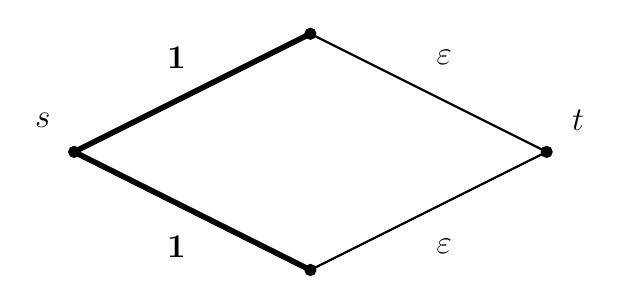
\begin{tikzpicture}[line cap=round,line join=round,>=triangle 45,x=1cm,y=1cm]
%\clip(-6.982493065694897,-13.63448020945784) rectangle (22.448157265896512,6.751180862658525);
\draw [line width=2pt] (0,0)-- (3,1.5);
\draw [line width=0.8pt] (3,1.5)-- (6,0);
\draw [line width=2pt] (0,0)-- (3,-1.5);
\draw [line width=0.8pt] (3,-1.5)-- (6,0);
\begin{scriptsize}\draw [fill=black] (6,0) circle (2pt);
\draw[color=black] (6.4,0.4) node {\large $t$};
\draw [fill=black] (0,0) circle (2pt);
\draw[color=black] (-0.4,0.4) node {\large $s$};
\draw [fill=black] (3,1.5) circle (2pt);
\draw [fill=black] (3,-1.5) circle (2pt);
\draw[color=black] (1.3,1.2) node {\large \bf{1}};
\draw[color=black] (4.7,1.2) node {\large $\varepsilon$};
\draw[color=black] (1.3,-1.2) node {\large \bf{1}};
\draw[color=black] (4.7,-1.2) node {\large $\varepsilon$};
\end{scriptsize}
\end{tikzpicture} 
\caption{Graph $G_1$}
\label{subfig:G_1}
\end{subfigure}
\begin{subfigure}[b]{0.48\columnwidth}
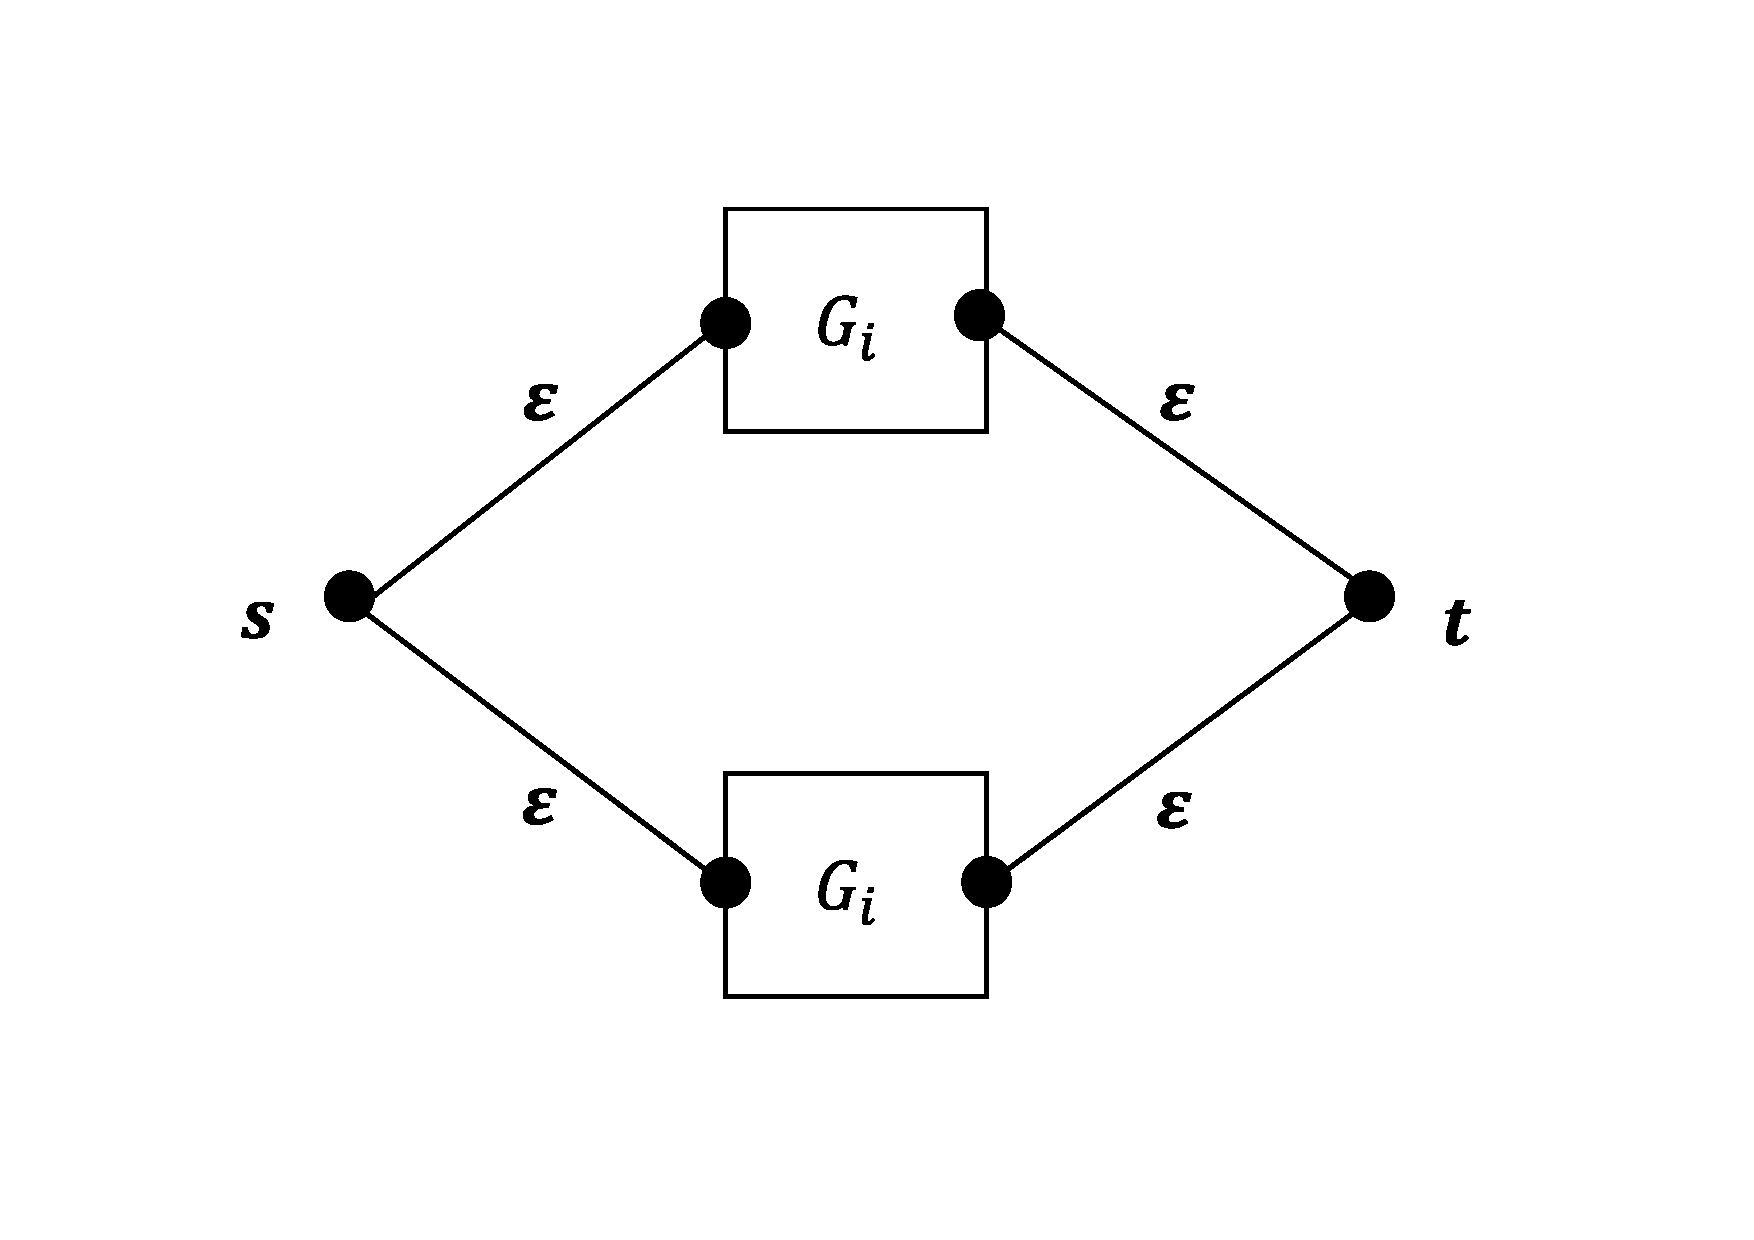
\includegraphics[scale=0.2]{G_i.pdf}
\caption{Graph $G_{i+1}$}
\label{subfig:G_i}
\end{subfigure}

%\begin{subfigure}[b]{0.48\columnwidth}
%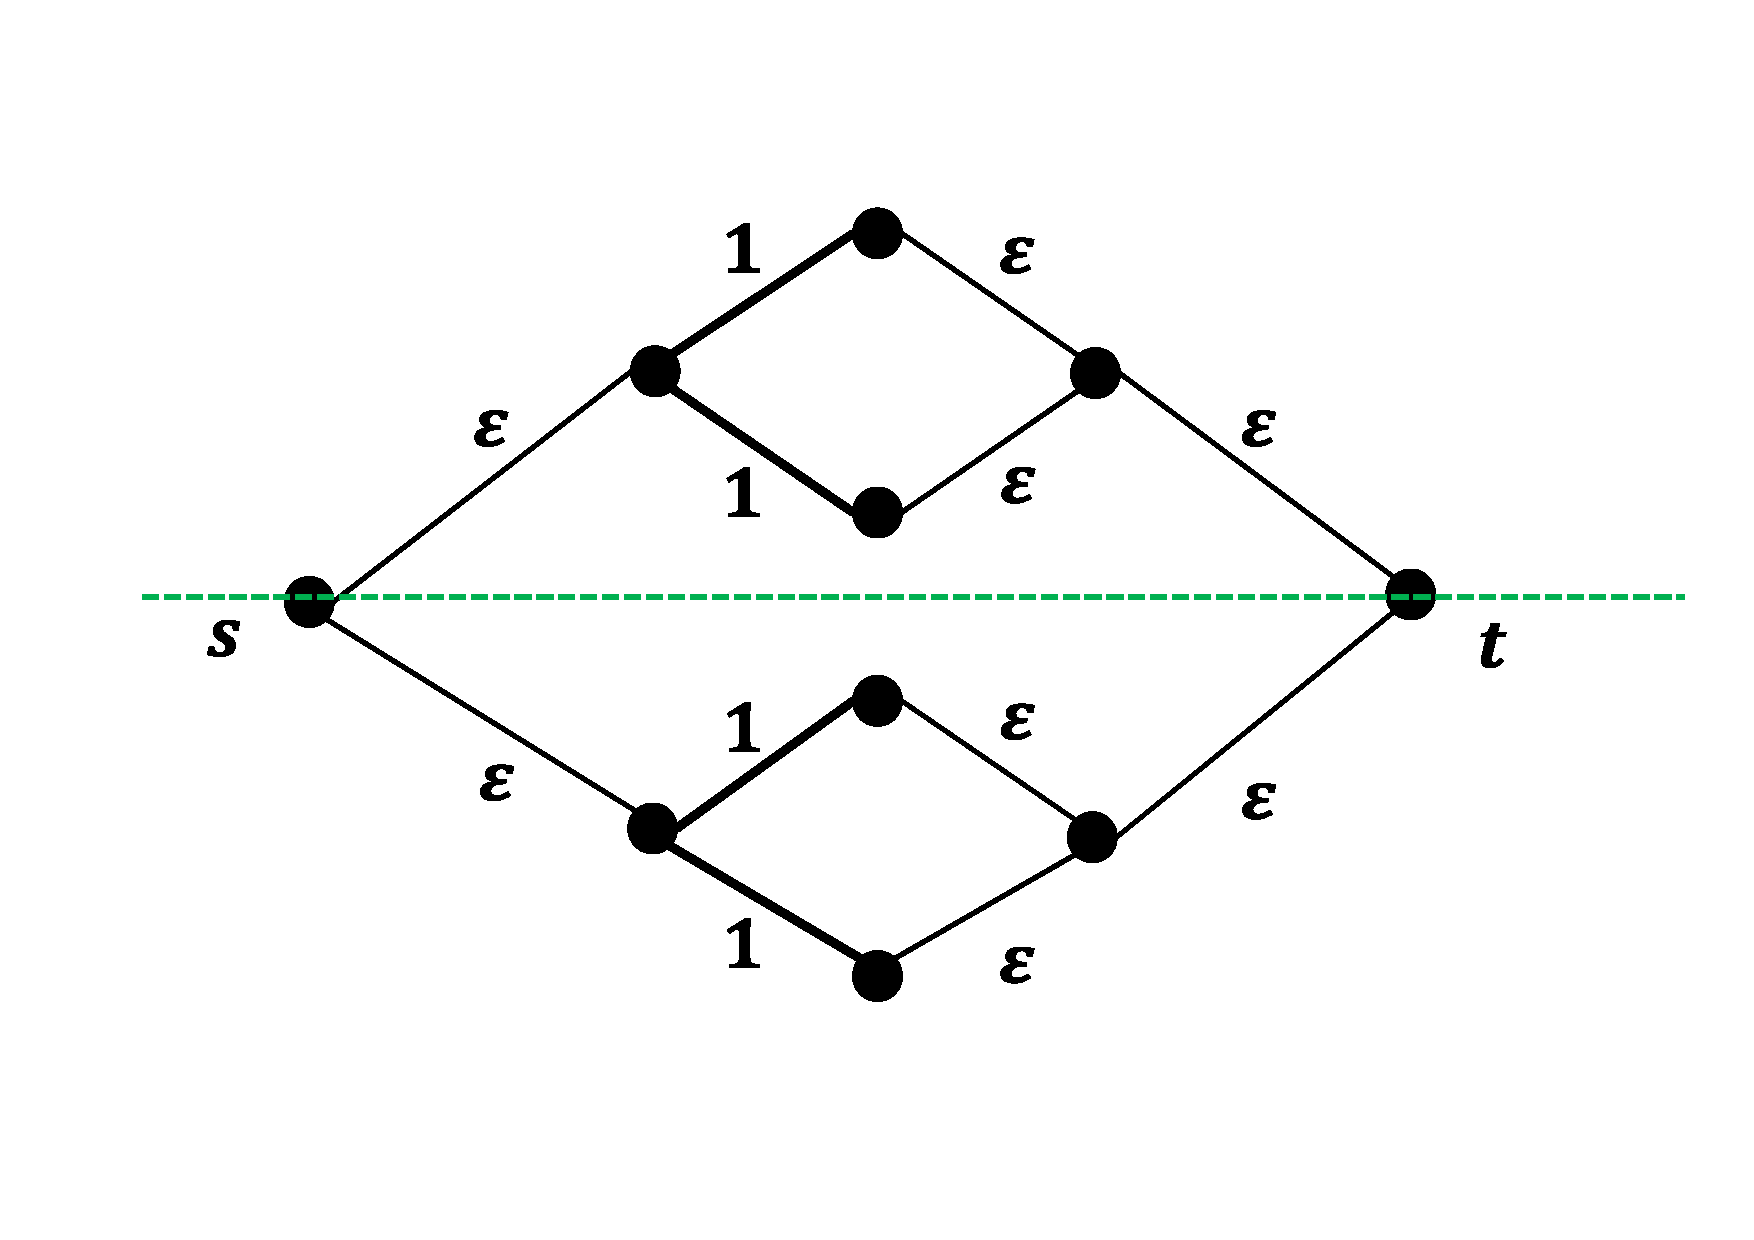
\includegraphics[scale=0.2]{G_2.pdf}\max\limits_{\substack{\mbox{\scriptsize{graph}} ~G\\ E_* \in \mcale_*}} c_A\left(G,E_*\right)
%\caption{Graph $G_2$ with the axis of symmetry}
%\end{subfigure}
%\begin{subfigure}[b]{0.48\columnwidth}
%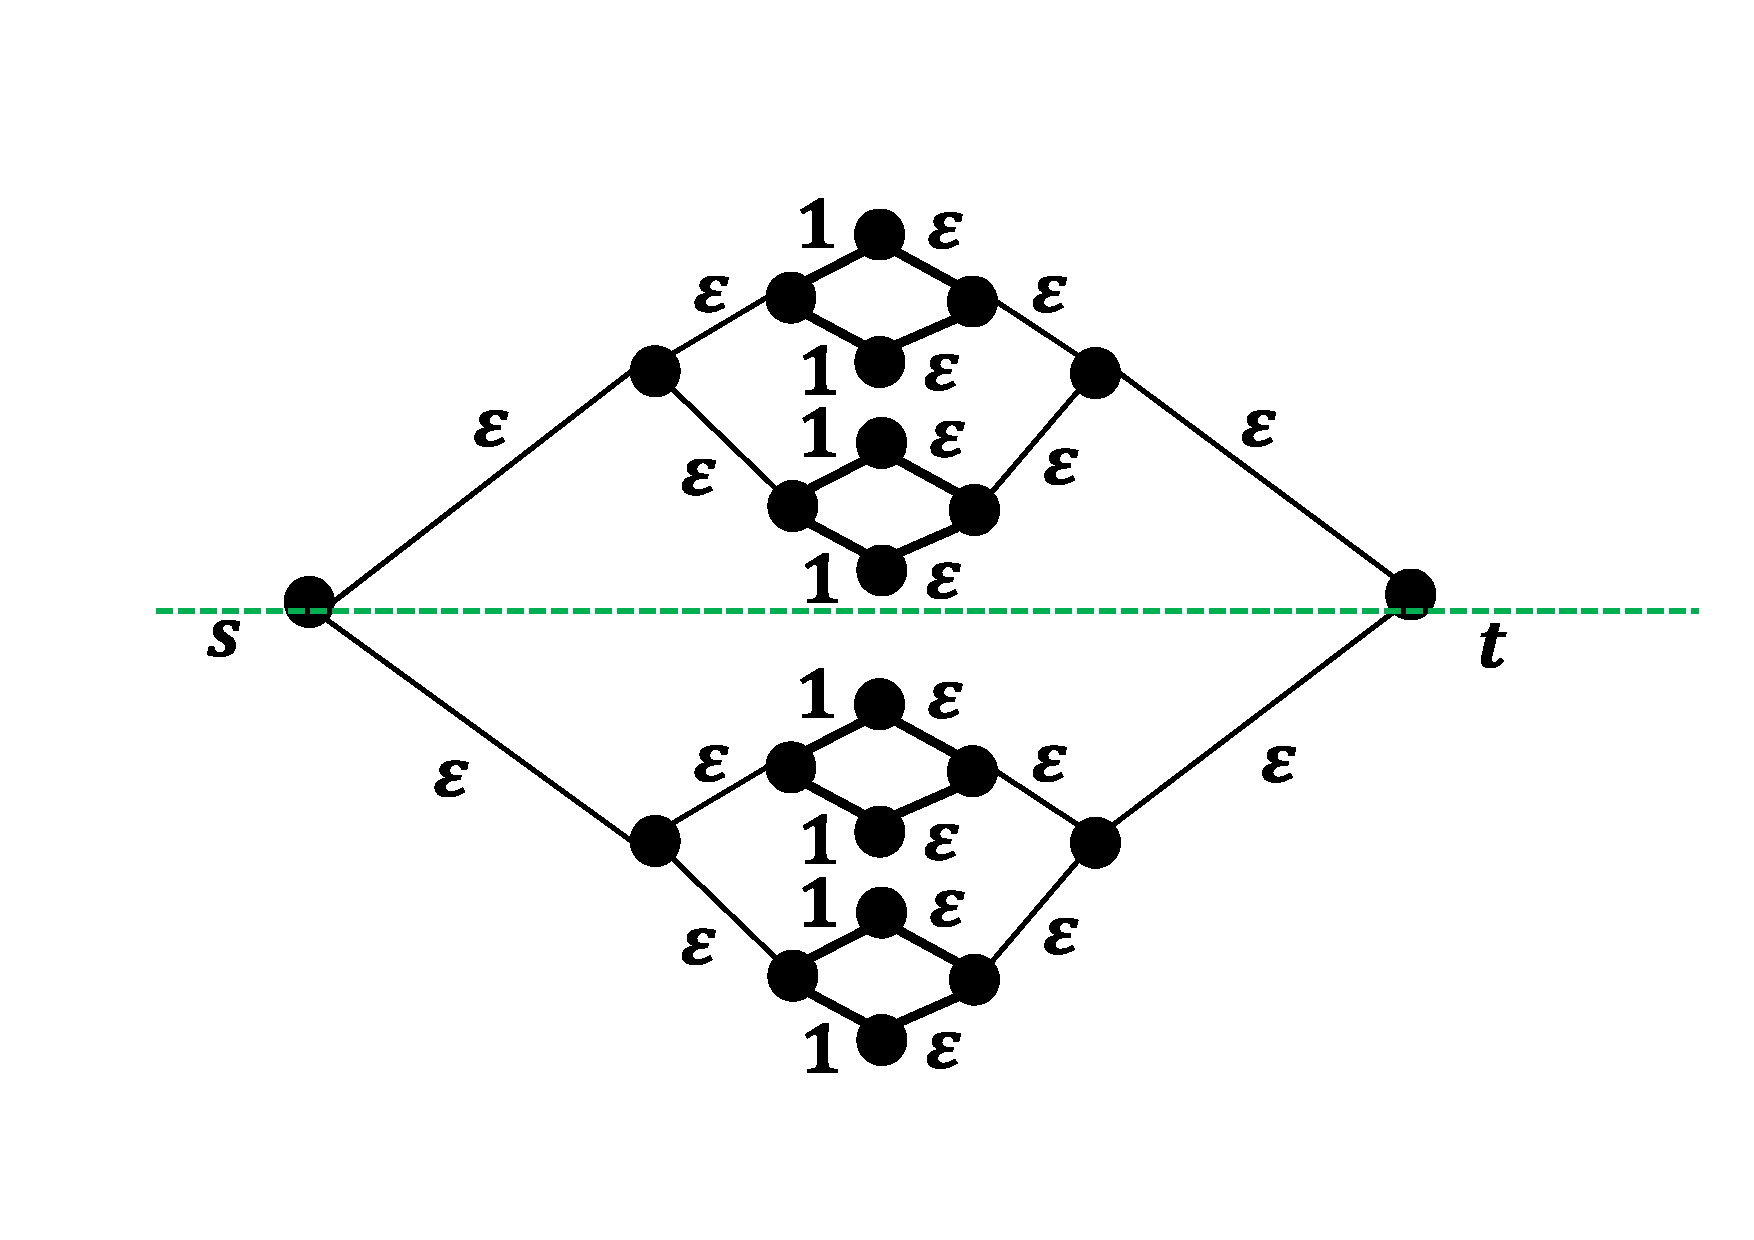
\includegraphics[scale=0.2]{G_3.pdf}
%\caption{Graph $G_3$ with the axis of symmetry}
%\end{subfigure}
\caption{Recursive construction of graphs $G_i$}
\label{fig:G_i}
\end{figure}

%\section{Conclusion and further work}

%We studied the competitiveness of the \mts es for the \kctp. In this context, an \mts ~is a strategy which does not make decisions referring to the anterior moves of the traveller, in other words, the nodes the traveller visited until his current position. We proved that the \textsc{comparison} strategy, defined in~~\cite{XuHuSuZh09}, is a \mts{}. This implies that the competitive ratio of the optimal deterministic \mts ~is $2k+1$. 

%Then, we constructed a series of \kctp{} instances, called road atlases and noted $\mcals_k$. Identifying an efficient randomized \mts{}es becomes harder when $k$ tends to infinity. We foremost concluded that a randomized  \mts{}~cannot reach a competitive ratio smaller than $\frac{10}{9}k+1 = 3.22(2)$ on road atlas $\mcals_2$. We extended our reasoning to larger atlases and established that the competitive ratio of randomized \mts es on maps with $k$ blockages is larger than $\left(3-\sqrt{3}\right)k + 1 \approx 1.268k+1$. That is to say that we identified an upper bound on the competitive ratio of randomized \mts{}es which is significantly higher than the existing one $k+1$. Now, if the objective is to find a strategy with a competitive ratio smaller than $k\beta + 1$, one shall study strategies which are not memoryless.

%The main issue that, in our opinion, needs further investigation, is the improvement of the new lower bound. There are, potentially, two ways to do this. The first one is the modification of road atlases $\mcals_k$ to make \mts es be less efficient on them. The second possibility consists in increasing the lower bound of the competitive ratio by introducing new properties of \mts es, more advantageous for bounding, on the road atlas $\mcals_k$. Other possible future work could be to design a randomized strategy with ratio less than $1.268k+1$ and which is not memoryless, or to design a family of maps such that there exists a randomized strategy which, applied on it, has a ratio $k+1$.
%Then, the difference of competitiveness between \mts es and other strategies is still open: is there a randomized strategy, which is not \mts , such that its competitive ratio is inferior to $\left(3 - \sqrt{3}\right)k+1$ ? We also wonder if there exists a randomized \mts ~whose competitive ratio is inferior to $2k+1$, which is the optimal competitive ratio of deterministic strategies.
% Another track is to study the competitiveness of randomized strategies (and particularly \mts es) on specific graphs, as Bender {\em et al.\/} did it with graphs composed of node-disjoint paths.

\bibliographystyle{plain}
\bibliography{mctp.bib}



\end{document}
